\subsection{Sequencing of a multivariable region and the problems that arise}

% Måste ha en bättre rubrik här och göra en bättre koppling till förra sektionen.
% Måste förklara varför jag skriver "more or less successfully sequenced"
In the previous section we talked about population genetics and showed some attempts to pinpoint the location of origin of a species. We showed that a number of studies on a large set of dogs leads to a single origin in South East Asia, but the hypothesis is not fully recognized by the scientific community. In this section we will describe how another experiment was perfomed, where a new genetic marker is studied in the same dataset as before.\\

\subsubsection{Sequencing process}

A 270 bp long exon of the gene DLA-DRB1 was sequenced in 3461 dogs. DLA-DRB1 was choosen for beeing the most variable part of mammalian genomes, and is therefore an excellent marker for population genetic studies(see earlier section). Genetic material was extracted and enriched in 14 PCR cycles and then prepared for sequencing by using a new technique described in \cite{neiman11} where a two tagging system made it possible to sequence up to 4992 samples in a single run. The actual sequencing was made using the 454 GS FLX Titanium Chemistry \cite{454_tech}, because of the length of the output reads from the 454 instrument. The perhaps more accurate Illumina instrument had a read length maximum of 100 high quality bases \cite{NextGen} at the time of the experiment, while the 454 instrument could produce read lengths of up to \textbf{500} bases \cite{454_problems}. With that length the whole exon of interest would fit in a single read, including primers. The most significant drawback of the 454 instrument is its problem with insertions and deletions, especially in homopolymeric regions \cite{454_problems}. We will show how this manifests in our data later.\\

% Skriv om demultiplexning. WHY?

Amplification of reads is a preparation that is necessary for all of the well used Massive Parallell Sequencing ({MPS}) instruments \cite{NextGen} and it is common that the {PCR} method \cite{pcr} is used. In short the sequence is extracted from the {DNA} in each individual and then labeled with two short tags for future identification. The two tagging system include one tag for the individual id and one for the plate id that the sequence is prepared on. After amplification the sequences are mixed, or pooled, and ready for sequencing. The sequence instrument has a maximum capacity of the number of reads that can be made in a run. These reads will be shared among the samples depending on how much sequence is available after amplification, with the result that some sample will get zero or very few reads and some samples will get a high coverage.\\

\subsubsection{Data}


Our data set consisted of a fasta file for each individual with between 20 and 425 reads. Data for individuals with fever reads was discarded since it was considered weak to draw any conclusion about the correct alleles. One read here means the 270 bp long exon with primer sequences, or tags, attached to both sides. The tags are known sequences with a length of 15 bp each. 
% Var kom dessa sekvenser ifrån, prata med Peter:
Moreover we had access to 113 published and soon to be published sequences (sequenced inhouse in an earlier project) of the same exon. These sequences had been validated by sanger sequencing \cite{sanger} and can be viewed as \emph{true} sequences, we'll call these \emph{reference sequences}.\\

Dog and wolf are, just like humans, diploid species which means that they have two copies of the genome in each cell, so if an individual have the same allele in both copies we say that this individual is \textbf{homozygote} for position \textbf{x}, and if there are two different alleles on the two copies we say that the individuale is \textbf{heterozygote} in this position. A collection of alleles is called a \textbf{haplotype} and one can be homozygote or heterozygote for a haplotype. In a diploid species there are not more than two alleles of a region, but in a population there can be many alleles.\\

\subsubsection{A closer look at the problems}

If there where no errors during the enrichment and sequencing process the data for one individual would consist of a number of identical sequences, if the individual was homozygote for the loci.\\
If the individual is a heterozygote we could expect a distribution where about half of the reads where identical to one variant and the rest to the other, as in figure \ref{fig:perfect_heterozygote}.

\begin{figure}[ht]
	\centering
		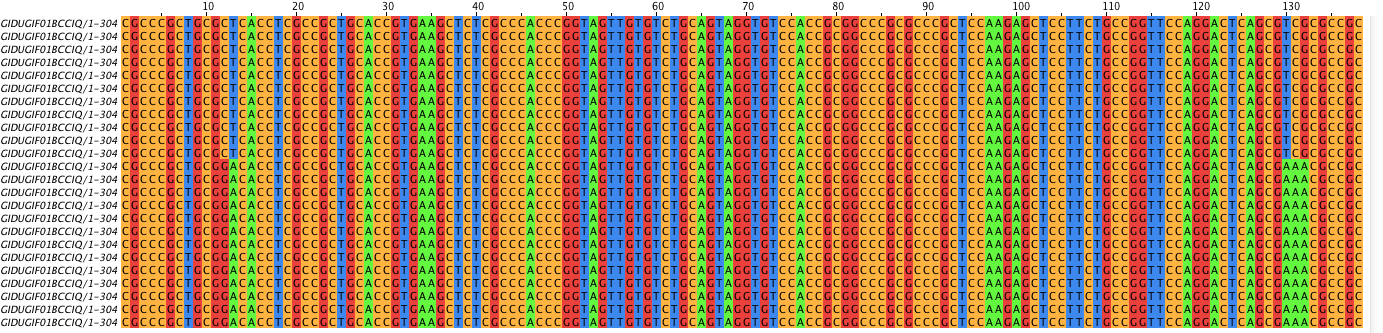
\includegraphics[width=0.8\textwidth]{../pictures/../pictures/perfect_heterozygote.png}
	\caption{Ideal Heterozygote: In this picture we can see that the 11 first reads show the sequence of one of the alleles, and the last 13 from the other. There is no ambiguities in the data, that is why we call it a perfect heterozygote. (Figure does not show the full length of the sequence.)}
	\label{fig:perfect_heterozygote}
\end{figure}

When the data is presented from the sequencer, many errors has arisen during the way, an example of real data can be seen in figure \ref{fig:align_chaos}.

\begin{figure}[ht]
	\centering
		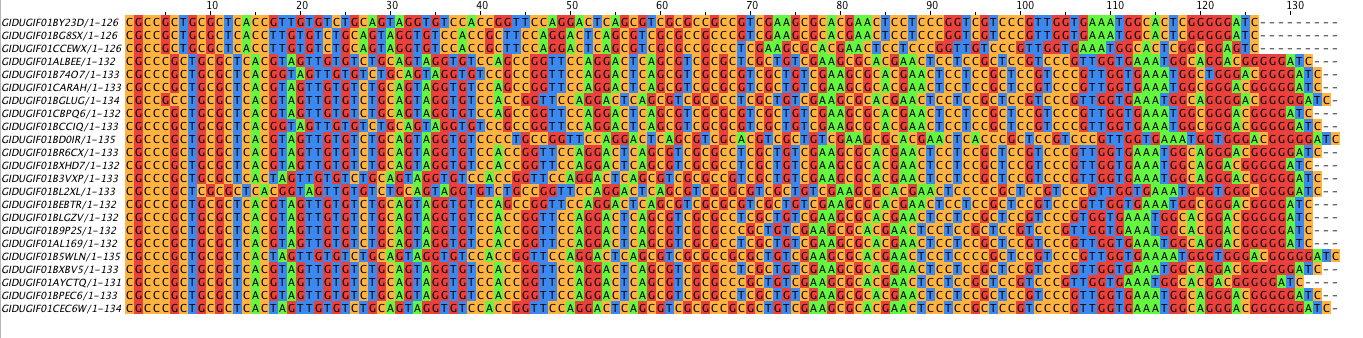
\includegraphics[width=0.8\textwidth]{../pictures/align_chaos_cropped.png}
	\caption{Actual Data: This is an example of how the true data looks like for a heterozygote dog. The lengths of the sequences varies as a result of the 454 instrument problems with homopolymeric regions \cite{454_problems}. (Figure does not show the full length of the sequence.)}
	\label{fig:align_chaos}
\end{figure}

We will now have a closer look at the different problems that can explain why figure \ref{fig:perfect_heterozygote} and figure \ref{fig:align_chaos} differs som much. To illustrate them we use a simplified figure, like figure \ref{fig:true_alleles}.

\begin{figure}[ht]
	\centering
		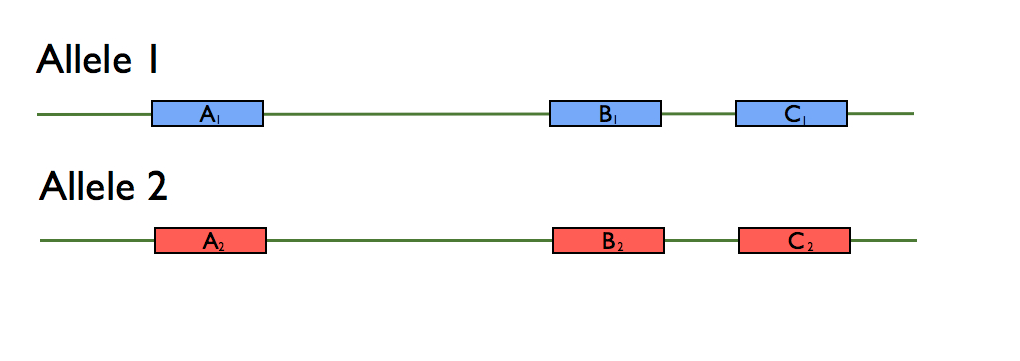
\includegraphics[width=0.7\textwidth]{../pictures/True_Alleles.png}
	\caption{Simplified sequence: This is a picture where we have collapsed the parts that are identical between the alleles, boxes represent positions where the alleles differ and the colours mark different variants.}
	\label{fig:true_alleles}
\end{figure}


\begin{itemize}
	\item \textbf{Single nucleotide variations}\\
	This is the case where the reads do not share the same base in a certain position. These variations can be true heterozygote variations or machine errors. If we trust that our alignment is correct this problem can be handled fairly simple since a true variation should be found in about half of the reads, like in figure \ref{fig:true_snv}. A read error is expected to be a random event and would therefore only be seen in a few number of reads as seen in figure \ref{fig:false_snv}.\\

	\begin{figure}[ht]
		\centering
			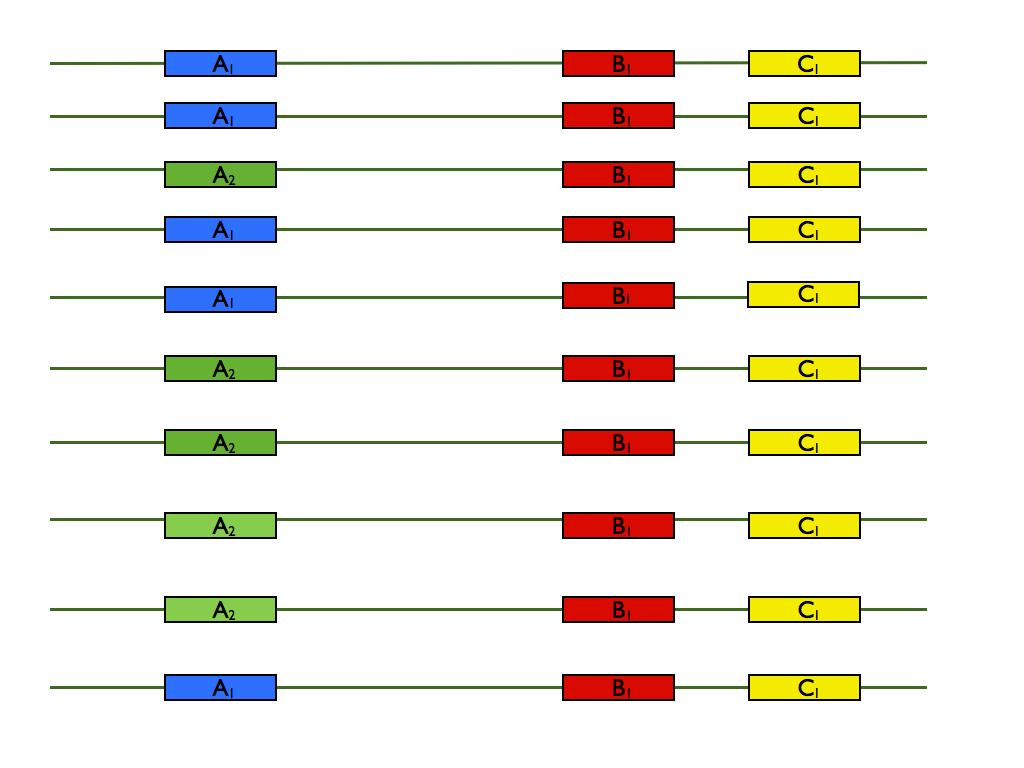
\includegraphics[width=0.5\textwidth]{../pictures/True_SNV.jpg}
		\caption{Expected pattern of a true SNV in simplified form, the variation appears in several reads.}
		\label{fig:true_snv}
	\end{figure}
	
	\begin{figure}[ht]
		\centering
			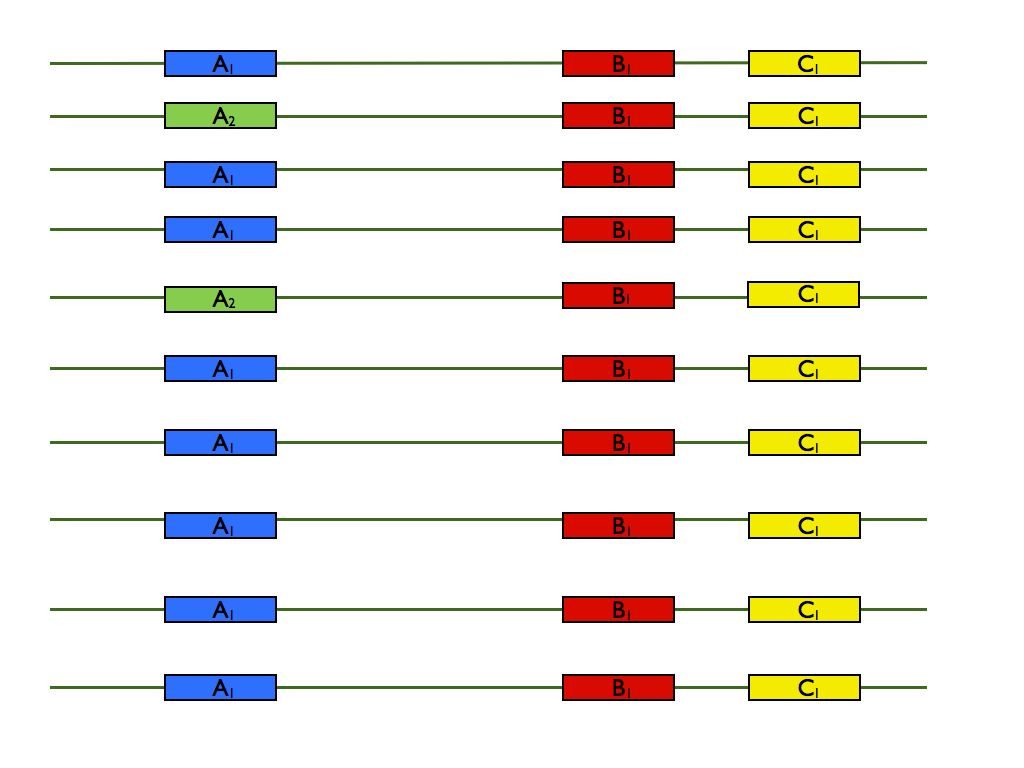
\includegraphics[width=0.5\textwidth]{../pictures/False_SNV.jpg}
		\caption{Expected pattern of a read error, the variation is rare or unique.}
		\label{fig:false_snv}
	\end{figure}
	
	\item \textbf{Insertion and deletions}\\
	Natural insertions or deletions (indels) in our sequence are highly unlikely. If the size of an indel is not a multiple of 3 it will cause a \emph{frameshift}. This means that the whole sequence of amino acids that the region is coding for after the indel will get displaced. A frameshift would most probably be lethal when occuring in such a vital part of the genome as this and combined with the fact that frameshift/nonframeshift indels in this region have not been observed in any of the published sequences we are not suspecting them to be true if observed in our data.\\
	
	The 454 instrument will, especially in homopolymeric regions, make false insertions and/or deletions, this is a well known drawback of this technology \cite{454_problems}. As an example of this problem we observed in our dataset that a conserved part of the sequence has a homopolymer with 5 consecutive C:s. We found that, out of all reads, 0.03\% had one C, 0.1\% two C:s, 30\% three, 56\% four and only 13\% showed all five C:s.	It might be true deletions but in this case it seems highly unlikely since all earlier observed reference sequences had 5 C:s in these positions.
	  
	\item \textbf{Chimeric sequences}
	Chimeric sequences can be thought of as artificial recombination and is formed during PCR amplification. When two segments from different {DNA} molecules are partially copied and added together, they give rise to false sequences that are very similar to the true alleles, example shown in figure \ref{fig:chimeric_sequences}. If a chimer is created in the early steps of the PCR they will show up in a large number of the reads for the individual, these are hard to handle. Our data was expected to include many chimeric sequences as a consequence of the large number of PCR cycles that was performed. This has been the hardest problem to handle of the ones mentioned.

	% Distinguish from real new alleles
	\begin{figure}[ht]
		\centering
			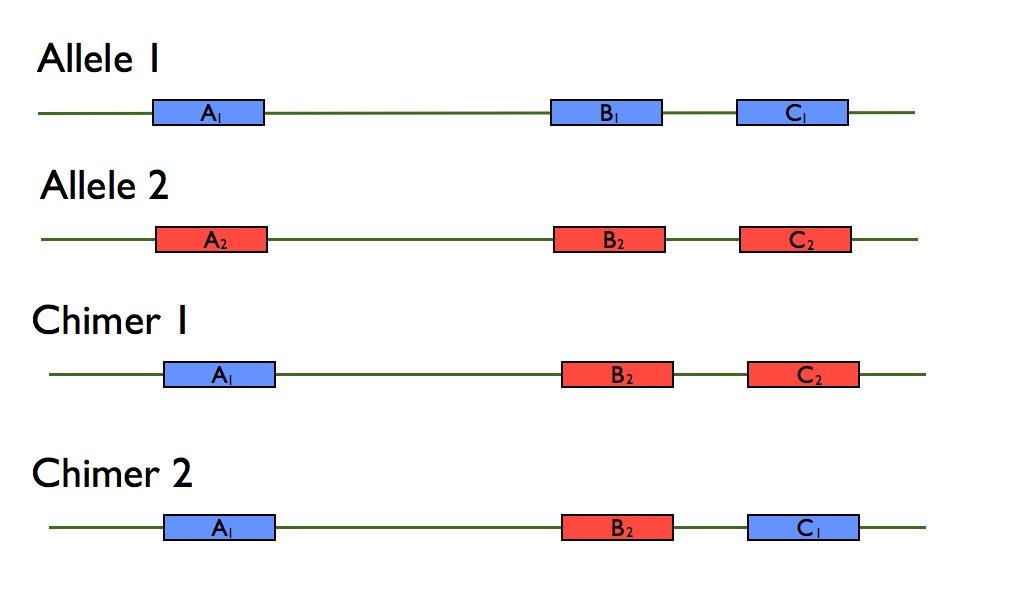
\includegraphics[width=0.7\textwidth]{../pictures/Chimers.jpg}
		\caption{Chimeric Sequences: The first two figures illustrates two alleles. Next we get two examples of how chimeric formations might look when segments from the true alleles, that include variations, have been partially copied and annealed together.}
		\label{fig:chimeric_sequences}
	\end{figure}

\end{itemize}


Since there are machine artifacts in the form of indels and read errors the first thing one would like to do is to align the reads so that they will be comparable, then we might be able to detect what is true variations and what is sequencing/PCR errors. In the next section we will see what methods we used to find the true sequences in our data.
